\section{实验四 IIR数字滤波器设计}

\subsection{一、实验目的}
1. 掌握模拟低通滤波器向数字低通滤波器的两种转换方法：冲激响应不变法、双线性变换法；
2. 区分模拟、数字滤波器的类型与时域、频域性能指标；
3. 学会使用MATLAB工具完成巴特沃斯模拟/数字滤波器设计；
4. 掌握滤波器冲激响应、幅频特性的仿真绘图与性能分析方法。

\subsection{二、实验原理}
1. IIR数字滤波器系统函数形式：
\[
H(z)=\frac{b_0+b_1z^{-1}+\dots+b_Mz^{-M}}{a_0+a_1z^{-1}+\dots+a_Nz^{-N}}
\]
设计核心为确定分子、分母系数，满足预设通带、阻带衰减指标。
2. 冲激响应不变法：对模拟滤波器冲激响应采样得到离散序列，实现$s\rightarrow z$映射；无频率畸变，但存在频谱混叠，不能用于高通、带阻滤波器设计。
3. 双线性变换法：映射公式
\[
s=\frac{2}{T}\frac{1-z^{-1}}{1+z^{-1}}
\]
$s$平面与$z$平面一一对应，无频谱混叠；存在频率预畸变，设计前需要对边界频率做预畸变校正。
4. 模拟原型法设计IIR滤波器通用流程：指标转换→估算阶数→构造模拟原型滤波器→s域转z域得到数字滤波器。

\subsection{三、实验内容}
1. 设计模拟巴特沃斯低通滤波器：通带截止300rad/s，阻带截止500rad/s，通带最大衰减3dB，阻带最小衰减20dB；绘制冲激响应、幅频特性曲线。
2. 冲激响应不变法设计数字巴特沃斯低通滤波器：$F_s=100\mathrm{Hz}$，$\omega_p=0.4\pi$，$\omega_s=0.8\pi$，$R_p=3\mathrm{dB}$，$R_s=15\mathrm{dB}$；绘制单位脉冲响应、幅频特性。
3. 双线性变换法设计同指标数字滤波器，做频率预畸变校正，与冲激不变法结果对比。

\subsection{四、实验结果}
\begin{figure}[H]
\centering
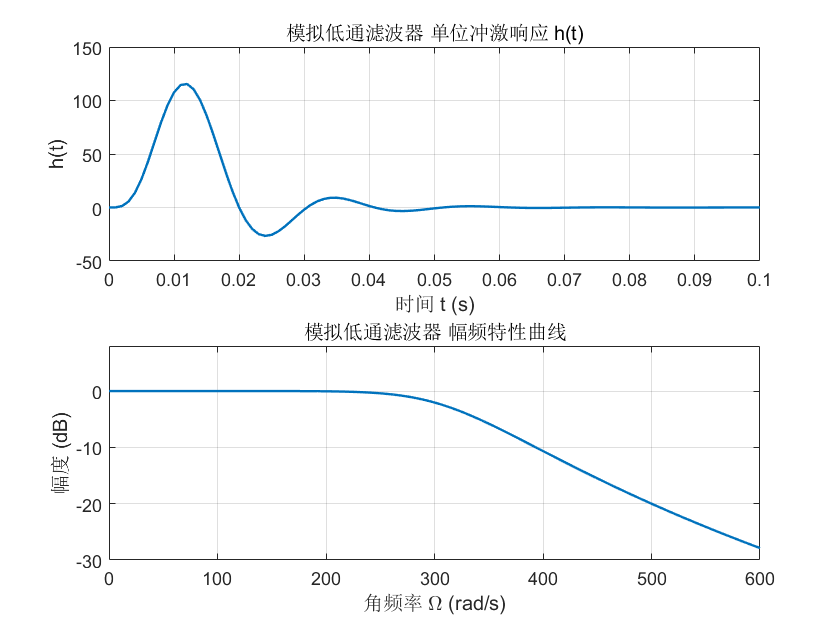
\includegraphics[width=0.9\textwidth]{4.1.png}
\caption{模拟巴特沃斯低通滤波器冲激响应与幅频特性}
\end{figure}

\begin{figure}[H]
\centering
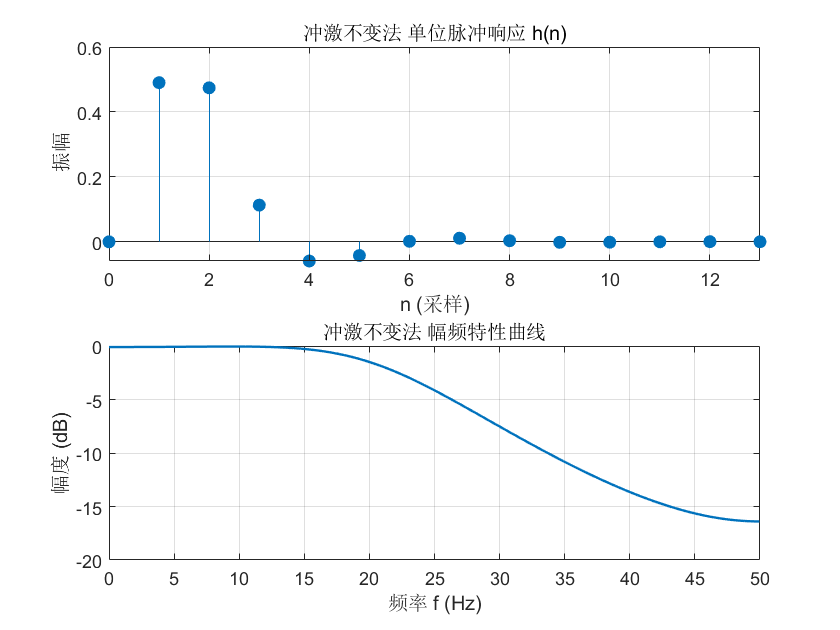
\includegraphics[width=0.9\textwidth]{4.2.png}
\caption{冲激响应不变法数字滤波器脉冲响应与幅频特性}
\end{figure}

\begin{figure}[H]
\centering
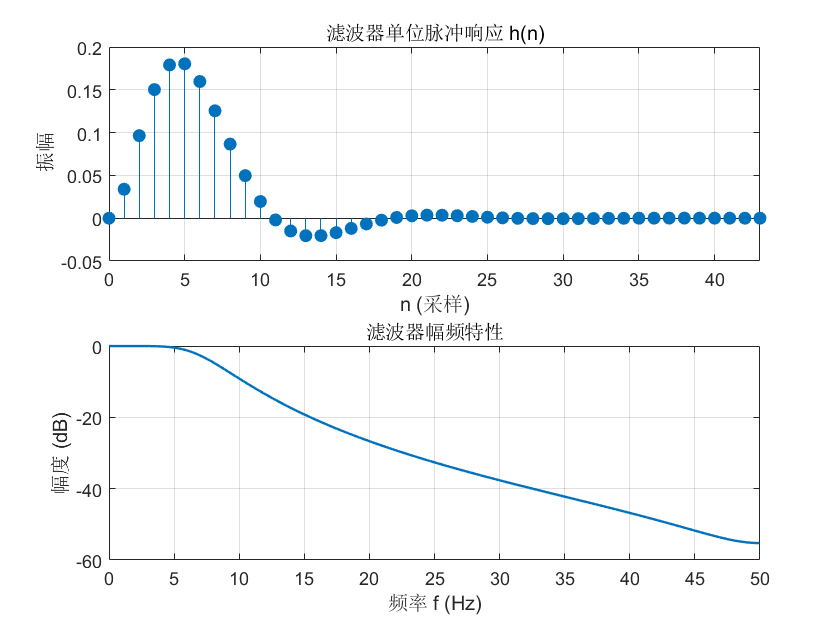
\includegraphics[width=0.9\textwidth]{4.3.png}
\caption{双线性变换法数字滤波器脉冲响应与幅频特性}
\end{figure}

\subsection{五、实验结论}
1. 模拟巴特沃斯滤波器幅频特性通带内平坦无波纹，阻带单调衰减，阶数由通带、阻带衰减指标唯一确定；时域冲激响应收敛稳定，符合因果系统要求。
2. 冲激响应不变法实现模拟到数字滤波器线性频率映射，无频率畸变，但高频存在频谱混叠，仅适用于低通滤波器；数字滤波器脉冲响应随时间衰减收敛。
3. 双线性变换法通过预畸变校正消除频率畸变，无频谱混叠，可设计任意类型滤波器；低频段两种方法滤波效果一致，高频段特性出现明显差异。
4. 仿真得到的幅频特性完全满足预设通带、阻带衰减指标，滤波器设计达标。

\subsection{六、完整MATLAB实验代码}
\subsubsection{exp4\_1.m 模拟巴特沃斯低通滤波器设计}
\begin{lstlisting}
%exp4_1.m 实验四 任务1：模拟巴特沃斯低通滤波器设计
%指标：通带截止300rad/s，阻带截止500rad/s，通带波纹3dB，阻带衰减≥20dB
clear;clc;close all;
%% ==========1. 滤波器性能指标赋值==========
Omega_p = 300;    %模拟通带截止角频率(rad/s)
Omega_s = 500;    %模拟阻带截止角频率(rad/s)
Rp = 3;           %通带最大衰减(dB)
Rs = 20;          %阻带最小衰减(dB)

%% ==========2. buttord求解滤波器最小阶数N、截止临界频率Wn==========
%带's'代表模拟滤波器设计
[n,Wn] = buttord(Omega_p,Omega_s,Rp,Rs,'s');
fprintf('模拟巴特沃斯滤波器阶数 n = %d\n',n);
fprintf('模拟滤波器临界截止角频率 Wn = %.2f rad/s\n',Wn);

%% ==========3. butter生成模拟滤波器分子b、分母a系数==========
[b,a] = butter(n,Wn,'s');

%% ==========4. tf构建系统传递函数H(s)，命令行输出==========
sys = tf(b,a);
disp('=========模拟滤波器系统传递函数 H(s)=========');
disp(sys);

% 新增：输出标准多项式分式形式
num_poly = poly2str(b,'s');
den_poly = poly2str(a,'s');
fprintf('\n========= 多项式分式形式 H(s) =========\n');
fprintf('H(s) = \n');
fprintf('        %s\n',num_poly);
fprintf('--------------------------------------------\n');
fprintf('        %s\n',den_poly);

%% ==========5. impulse求解0~0.1s冲激响应h(t)==========
t = 0:0.001:0.1;   %时间轴：步长0.001s，范围0~0.1s
h_t = impulse(b,a,t);

%% ==========6. freqs求解0~600rad/s幅频特性==========
f_axis = 0:1:600;  %频率轴范围0~600rad/s
[H_s,freq] = freqs(b,a,f_axis);
mag_dB = 20*log10(abs(H_s)); %幅度转换为dB

%% ==========7. 分2行绘图：冲激响应+幅频特性==========
figure('Name','exp4_1 模拟低通滤波器');
%子图1：时域冲激响应
subplot(2,1,1);
plot(t,h_t,'LineWidth',1.2);
title('模拟低通滤波器 单位冲激响应 h(t)');
xlabel('时间 t (s)');
ylabel('h(t)');
grid on;

%子图2：频域幅频特性，约束坐标axis([0 600 -30 8])
subplot(2,1,2);
plot(f_axis,mag_dB,'LineWidth',1.2);
title('模拟低通滤波器 幅频特性曲线');
xlabel('角频率 \Omega (rad/s)');
ylabel('幅度 (dB)');
axis([0 600 -30 8]); %严格遵照指导书坐标轴范围
grid on;
\end{lstlisting}

\subsubsection{exp4\_2.m 冲激响应不变法设计数字低通滤波器}
\begin{lstlisting}
%exp4_2.m 冲激响应不变法设计巴特沃斯数字低通，严格匹配本题指标
clear;clc;close all;
%% 1. 参数设置（严格按题目给定）
Fs = 100;    %采样频率Hz
T = 1/Fs;
wp = 0.4*pi;    %数字通带截止角频率 rad
ws = 0.8*pi;    %数字阻带截止角频率 rad
Rp = 3;      %通带最大衰减dB
Rs = 15;     %阻带最小衰减dB

%% 2. 数字角频率转模拟角频率 Ω=ω/T（冲激响应不变法线性映射）
Omega_p = wp / T;
Omega_s = ws / T;

%% 3. buttord求模拟滤波器最小阶数n和截止频率Wn
[n, Wn] = buttord(Omega_p, Omega_s, Rp, Rs, 's');
fprintf('模拟巴特沃斯原型阶数 n = %d\n',n);

%% 4. butter设计模拟低通H(s)
[b_s, a_s] = butter(n, Wn, 's');

%% 5. impinvar做s→z变换得到数字滤波器系数
[bz, az] = impinvar(b_s, a_s, Fs);

%% 6. tf生成离散系统传递函数H(z)
sys_z = tf(bz, az, T);
disp('=====数字滤波器系统函数H(z)=====');
disp(sys_z);
% 输出分式形式方便报告抄写
num_p = poly2str(bz,'z');
den_p = poly2str(az,'z');
fprintf('\nH(z)分式形式：\nH(z) = %s / (%s)\n',num_p,den_p);

%% 7. 分2行绘图：脉冲响应 + 幅频特性
figure('Name','冲激响应不变法数字低通滤波器');
% 子图1：impz绘制脉冲响应
subplot(2,1,1);
impz(bz,az);
title('滤波器单位脉冲响应 h(n)');
grid on;

% 子图2：freqz求频响，横轴转Hz、纵轴转dB
subplot(2,1,2);
[H, w] = freqz(bz, az, 1024); %w范围0~π归一化角频率
mag_dB = 20*log10(abs(H));
f_Hz = w/(2*pi)*Fs; % 归一化角频率→真实频率Hz
plot(f_Hz, mag_dB, 'LineWidth',1.2);
title('滤波器幅频特性');
xlabel('频率 f (Hz)');
ylabel('幅度 (dB)');
grid on;
\end{lstlisting}

\subsubsection{exp4\_3.m 双线性变换法设计数字低通滤波器（含预畸变）}
\begin{lstlisting}
%exp4_3.m 双线性变换法 带频率预畸变设计数字低通滤波器
clear;clc;close all;
Fs = 100;
T = 1/Fs;
wp = 0.4*pi;
ws = 0.8*pi;
Rp = 3; Rs = 15;

%% 频率预畸变校正
Omega_p = (2/T)*tan(wp/2);
Omega_s = (2/T)*tan(ws/2);

%% 设计模拟原型滤波器
[n,Wn] = buttord(Omega_p,Omega_s,Rp,Rs,'s');
[b_s,a_s] = butter(n,Wn,'s');

%% 双线性变换 s->z
[bz,az] = bilinear(b_s,a_s,Fs);

%% 输出传递函数
sys_z = tf(bz,az,T);
disp('=====双线性变换法 H(z)=====');
disp(sys_z);

%% 绘图
figure('Name','双线性变换法数字低通');
subplot(2,1,1);
impz(bz,az);
title('单位脉冲响应 h(n)');
grid on;

subplot(2,1,2);
[H,w] = freqz(bz,az,1024);
mag_dB = 20*log10(abs(H));
f_Hz = w/(2*pi)*Fs;
plot(f_Hz,mag_dB,'LineWidth',1.2);
title('幅频特性曲线');
xlabel('频率 f(Hz)');
ylabel('幅度(dB)');
grid on;
\end{lstlisting}